\section{Jump Points}
In the previous section we developed simple rules for pruning neighbours during 
individual node expansions. We now extend this idea in order to define a 
macro-step operator which speeds up optimal search by selectively expanding
only certain nodes on a grid map. We term these nodes \emph{jump points}.
\par
The basic idea is straightforward: we give a simple example in Figure 
\ref{fig:jumppoints}(a).
Here we observe that when moving straight there are many cases where
the expanded node has only a single successor.
Since this successor cannot improve any other nodes on the open list we 
propose to evaluate it immediately, thereby avoiding an unnecessary list
maintenance operation. 
If we keep moving in the same direction we can continue this process until we 
either reach a node with more than one successor (a jump point), which we add to the open list instead of the nodes whose evaluation we expedited, or we find an 
obstacle which indicates that further search in this direction is fruitless.
\par
In the remainder of this section we will develop a macro-step operator which 
speeds up node expansion by identifying jump point successors in the case of
both straight and diagonal moves. We begin by making precise the concept of a
jump point:

\begin{definition}
\label{def:jump}
A node $x$ is designated a jump point if it satisfies at least one of the following
conditions:
\begin{enumerate}
\item{$x$ is a node which, after pruning, is adjacent to at least one neighbour
whose evaluation is forced according to the rules in Section
\ref{sec:prunestraight} and Section \ref{sec:prunediagonal}.}
\item{$x$ is located on the same row or column of the grid as the goal.}
\item{$x$ has one or more successors which are themselves jump points.}
\end{enumerate}
\end{definition}

Note that we distinguish between a neighbour, which is immediately adjacent to
$x$ on the grid, and a successor which may not be. 
This is a fine but important distinction as in our work a neighbour can be a 
successor but the converse is not necessarily true.
Thus, when expand $x$, we will only consider its successors.


\subsection{Generating Successors}
The process by which we generate the set of successors necessary to expand a
node $x$ is given in Algorithm \ref{alg:successors}.
We start with the pruned set of neighbours immediately adjacent to $x$ (line 2).
Then, instead of immediately adding each neighbour $n$ to the set of successors
for $x$, we try to ``jump'' to a node that is further away but which lies in the 
same relative direction to $x$ as $n$ (lines 3:4). 
For example, if the edge $(x, n)$ constitutes a
straight move travelling \emph{right} from $x$, we look for a jump point among
the nodes immediately to the right of $x$.
If we find such a node, we add it to the set of successors instead of $n$.
In the case where we fail to find a jump point, we add nothing.
The process continues until the set of neighbours for $x$ is exhausted.

\input alg_jumpexpansion

\subsection{Jumping}
The process by which we identfy jump points is given in Algorithm
\ref{alg:jump}; it requires an initial node $x$, a direction of travel $dir$
(e.g. up, down, left right, etc) and the goal node $g$.
In rough overview, the algorithm attempts to establish whether $x$ has any 
jump point successors by stepping in the direction $dir$ and testing
if the node $n$ at that location satisfies the constraints outlined in 
Definition \ref{def:jump}.
When this is the case, $n$ is designated a jump point and returned (lines 5, 7
and 11).
When $n$ is not a jump node the algorithm recurses and steps again in direction
$dir$ but this time $n$ is the new initial node (line 12).
The recursion terminates when an obstacle is encountered and no further
steps can be taken (line 3).
Note that before each diagonal step the algorithm must first 
fail to detect any straight jump points (lines 9:11). 
This check corresponds to the third constraint of Definition \ref{def:jump} 
and is essential for preserving optimality.
We give an example of diagonal jump point identification in Figure
\ref{fig:jumppoints}(b).

\begin{figure}[tb]
       \begin{center}
		   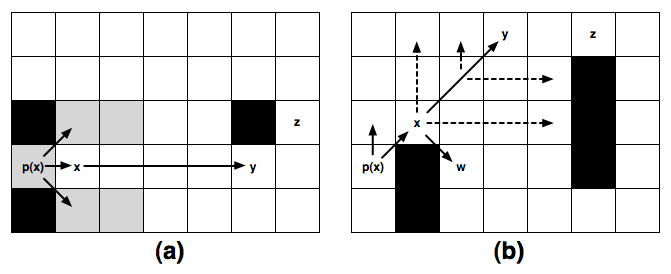
\includegraphics[scale=0.35, trim = 10mm 10mm 10mm 0mm]
			{diagrams/jumppoints.png}
       \end{center}
	\vspace{-3pt}
       \caption{Examples of straight (a) and diagonal (b) jump points.
Dashed lines indicate a sequence of interim node evaluations that reached
a dead end. Strong lines indicate eventual successor nodes.}
       \label{fig:jumppoints}
\end{figure}

\subsection{Optimality}
In this section we prove that for each optimal length path in a grid map there
exists an equivalent length path which mentions only jump points (Theorem
\ref{theorem:jumpoptimal}).  Our result is derived by splitting each optimal 
length path into contiguous segments and identifying special nodes along each segment 
called \emph{turning points}.

\begin{definition}
A \emph{turning point} is any node $n_{i}$ along a path where the direction of
travel from the previous node $n_{i-1}$ to $n_{i}$ is different to the direction
of travel from $n_{i}$ to the subsequent node $n_{i+1}$.
\end{definition}

Before proving our main result, we will first derive an interim result that
in which we show jumping from one jump point node to any other is optimal.

\begin{lemma}
\label{lemma:jumping}
For each optimal length path between two jump point nodes on a grid there exists
an equivalent length path that mentions only jump point nodes.
\end{lemma}
\begin{proof}
Let $\pi$ be an arbitrarily chosen optimal path between two jump point nodes
on a grid.  
%We will show that for each $\pi$ there exists a symmetric path $\pi'$ which has
%the same length and mentions only nodes that are jump points.
\par
First, divide the optimal path into a series of adjacent
segments s.t. $\pi = \lbrace \pi_{0}, \ldots, \pi_{n} \rbrace$. Each $\pi_{i} 
= \lbrace n_{k}, n_{k+1}, \ldots, n_{l-1}, n_{l} \rbrace$
is a subpath comprised of one or more contiguous steps in the same
direction (e.g.  only steps ``up'' or ``down'' etc).  Next, rewrite $\pi$ to
minimise the number of segments.  This is a greedy procedure which we
outline in Algorithm \ref{alg:segments}; the idea is to rewrite $\pi$ s.t steps
in one direction, when possible, are taken together rather than interleaved with
steps in a second direction (e.g. ``up'', ``up'', ``right'' instead of ``up'',
``right'', ``up'').  
%After rewriting $\pi$, each node at the beginning and end
%of a segment $\pi_{i}$ is a turning point where the optimal path is forced to change
%direction. If this were not true, we could continue rewriting $\pi$ until it is.
\par
Since each $\pi_{i}$ consists only of moves in a single direction
(straight or diagonal) we can construct an equivalent segment $\pi'_{i}$ that
mentions only the turning point nodes at the start and end of each $\pi_{i}$.
Clearly the length of $\pi'_{i}$ is optimal.
It remains to show only that we expand each node mentioned by every $\pi'_{i}$.
Notice that, with the exception of the start and goal, each such node is also a 
turning point. 
By Corollary \ref{corollary:turningpoints} each turning point is 
also a jump point, so every turning point node must be expanded during search.
Only the start and goal remain. These are jump points by definition and must
also be expanded.
We thus construct $\pi' = \lbrace \pi'_{0}, \ldots, \pi'_{n}\rbrace$. Since each
$\pi'_{i}$ is equivalent to each $\pi_{i}$, it follows that $\pi'$ is equivalent
to $\pi$ and thus optimal.
\end{proof}

\begin{corollary}
\label{corollary:turningpoints}
Each turning point along a path returned by Algorithm \ref{alg:segments} is
also a jump point.
\end{corollary}
\begin{proof}
A proof will go here. It will spell out that each turning point is either
located next to an obstacle or has a jump point successor.
\end{proof}

\input alg_segments

\begin{theorem}
\label{theorem:jumpoptimal}
Searching with jump points is optimal.
\end{theorem}
\begin{proof}
Let $s$ and $g$ be arbitrarily chosen locations on a grid that represent
and goal location associated with a particular pathfinding query.
By definition $s$ is a jump point. Since it has no parent we jump in every 
allowable direction away from $s$ computing all possible jump point successors.
By Lemma \ref{lemma:jumping} we can travel optimally from the
successors of $s$ to any other jump point on the grid.
Since the goal $g$ is a jump point by definition, it follows that an optimal
length path from $s$ to $g$ is returned.
\end{proof}

